\begin{figure}[!]
    \centering
    \begin{subfigure}{\textwidth}
    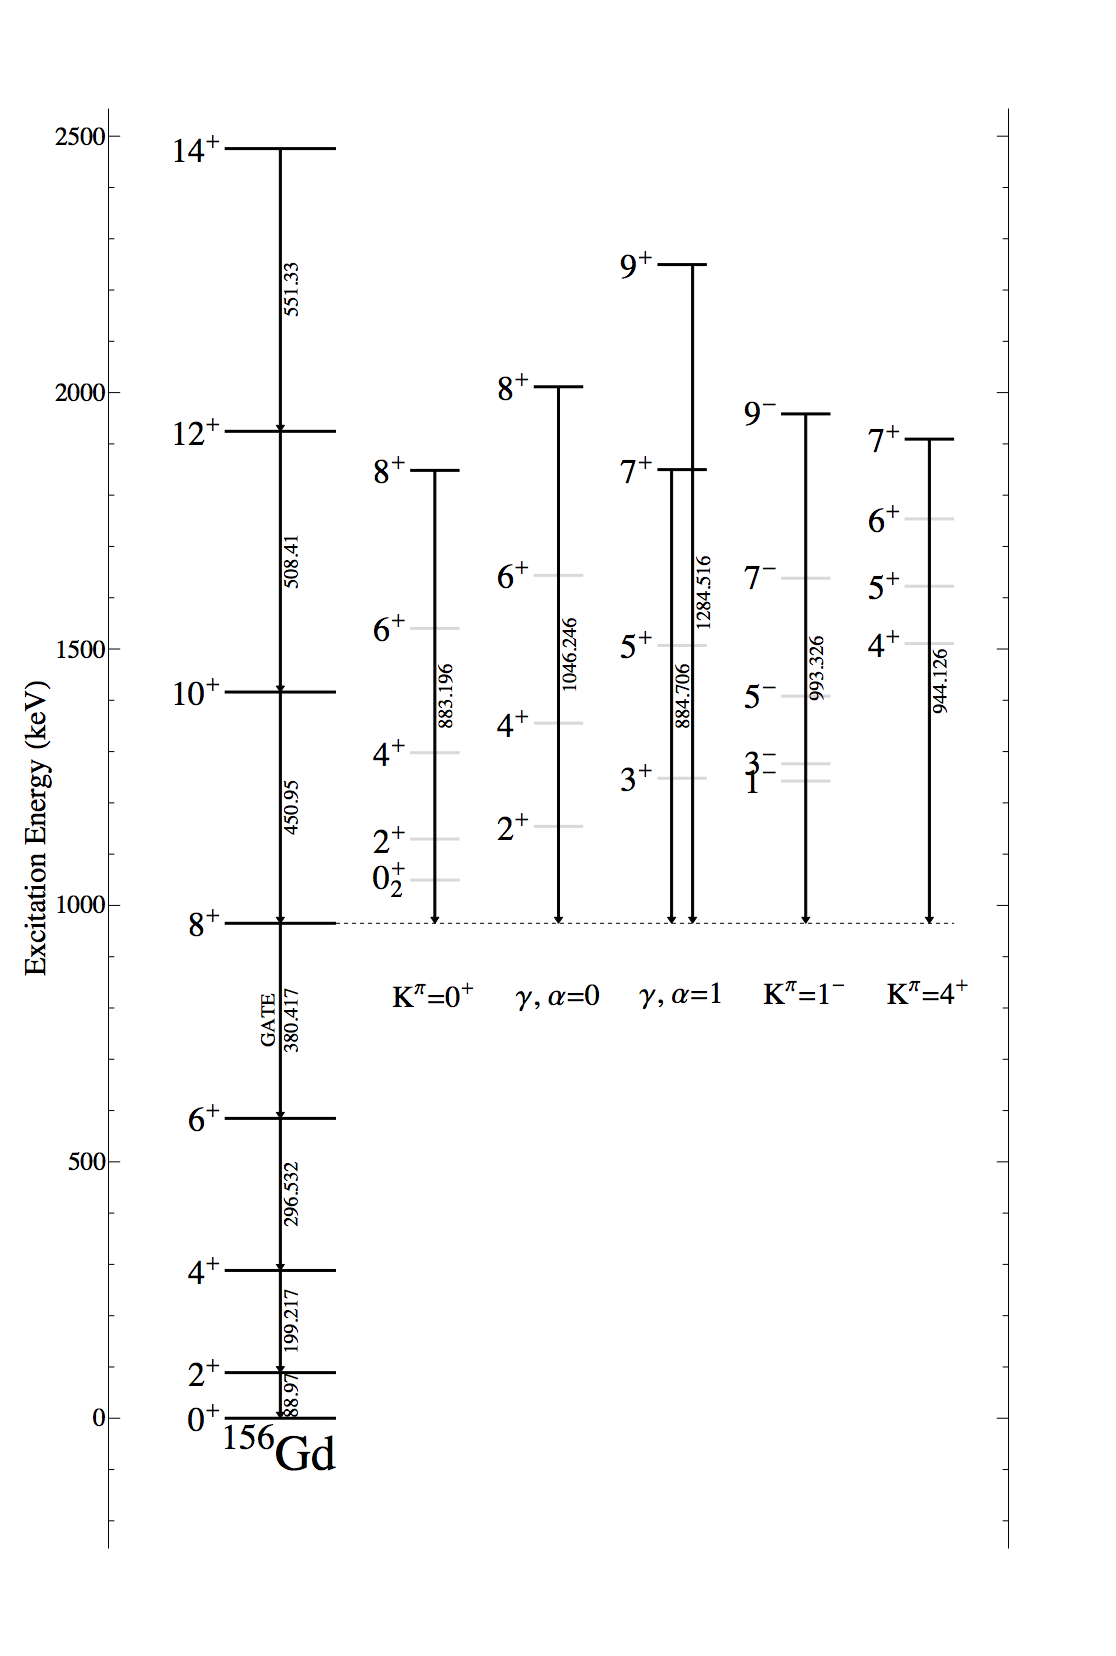
\includegraphics[scale=0.35]{156GdTablesAndFigs/156Gd_8to6.eps}
    \caption{\label{fig:156_8to6level}Level Scheme of $^{156}$Gd. The gamma ray of the $8^+$\rightarrow$6^+$ (380 keV) transition in the ground state was gated on. It was then compared with the gated spectrum from the gamma ray of the $10^+$\rightarrow$8^+$ (451 keV) transition in the ground state. Peaks only appearing in the first gate were assumed to go into the $8^+$ state, and assignments were made. Additionally, these peaks were also gated on, to look for cascades leading into the $8^+$ state, which were found in several cases. The levels are organized by band. The lower levels of the band, unseen by gamma rays in this gate, are in gray.}
    \end{subfigure}
    \captionlistentry{Level scheme and spectrum of $^{156}$Gd based on the $8^+\rightarrow6^+$ transition.}
    \label{fig:156_8to6}
    \end{figure}
\begin{landscape}
    \begin{figure}
    \ContinuedFloat
    \begin{subfigure}{1.4\textwidth}
    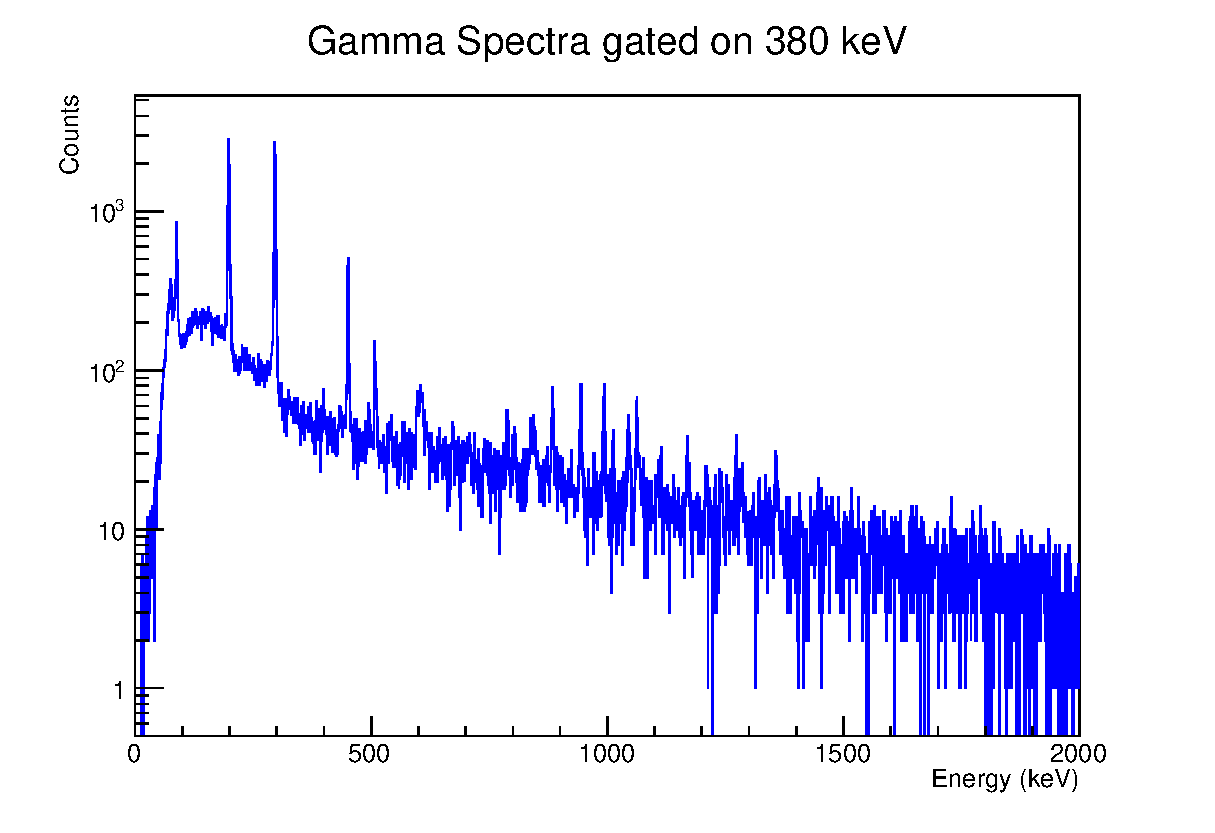
\includegraphics[]{156GdTablesAndFigs/380GateSpectrum.eps}
    \caption{Gamma spectrum gated on 380 keV, corresponding to the $8^+\rightarrow6^+$ transition.}
    \label{fig:156_8to6spec}
    \end{subfigure}
\end{figure}
\end{landscape}